\begin{figure}[htp]
\centering
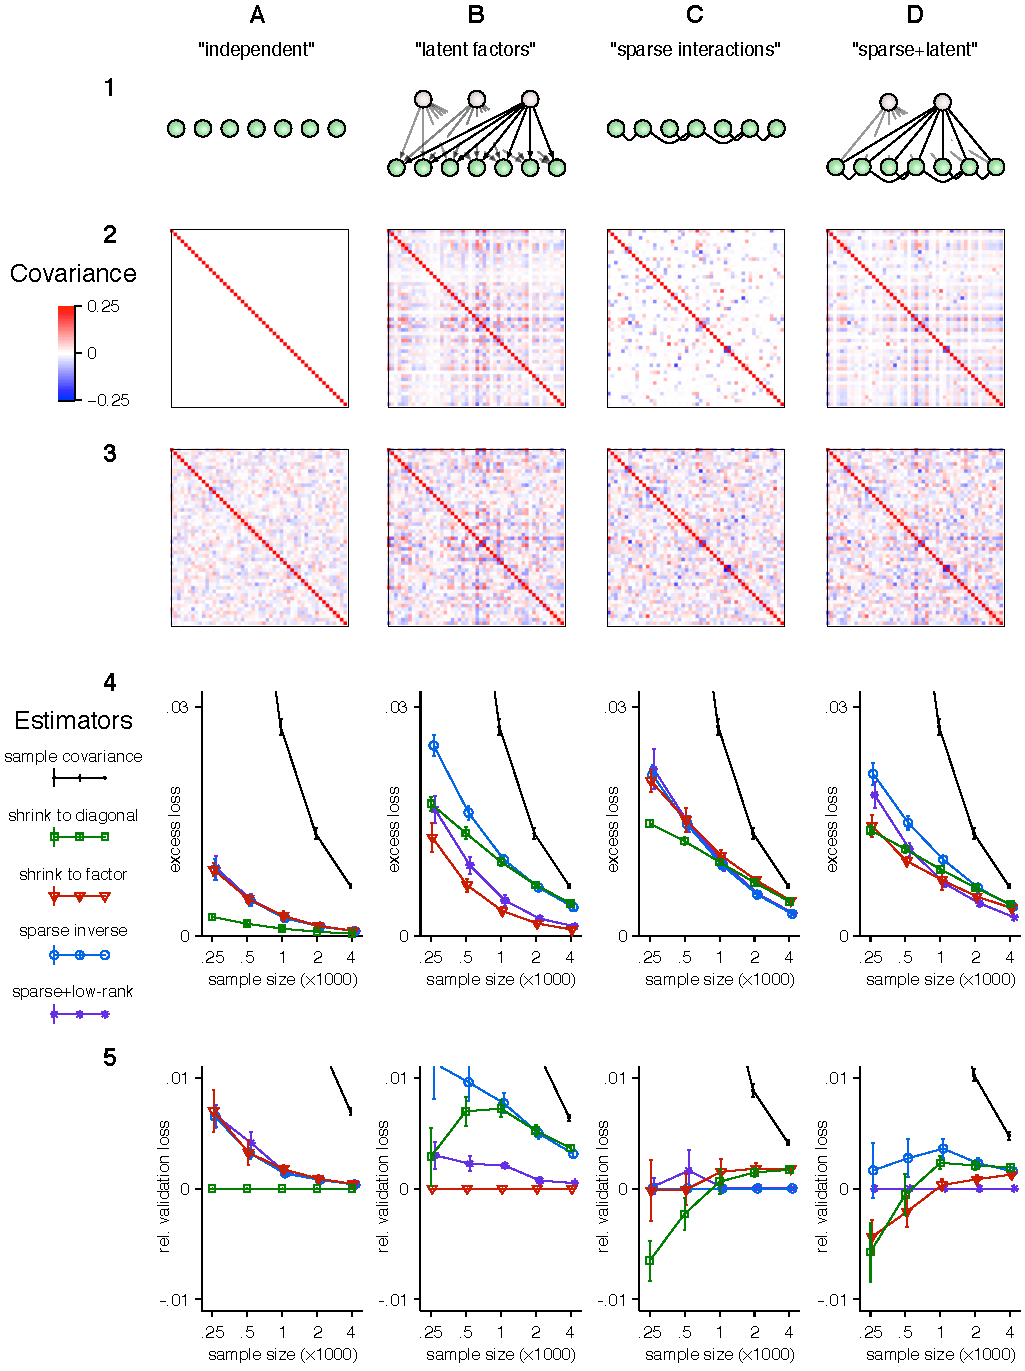
\includegraphics{figures/Simulation.pdf}
\caption{
Graphical models corresponding to the low-dimensional targets of the four regularization schemes used in the paper. It assumed that all interactions are linear, \emph{i.e.}\;the mean firing rate of any neuron can be computed by a linear combination of the firing rates of other neurons and latent units.
\textsf{A}: ``Independent.'' A population with no interactions corresponds to the diagonal covariance matrix.
\textsf{B}: ``Latent factors.'' Observed nodes are assumed to be influenced by several latent units (``factors") but are otherwise independent.
\textsf{C}: ``Sparse.'' Partial correlations between a subset of pairs of observed neurons, zero partial correlations between all other pairs.  
\textsf{D}: ``Sparse+latent.''  Partial correlations between a subset of pairs of observed neurons and a few latent factors interacting with the entire population. 
{\sf E--H} are examples of true $100\times100$ covariance matrices of multivariate normal distributions used in simulations. Matrix A has no low-dimensional structure. Matrices B--D have low-dimensional structture corresponding to the respective graphical models in Fig.~2B--D.
{\sf I--L} are examples of sample covariance matrices obtained from samples of size $n=1000$ from distributions with respective true covariance matrices A--D.
{\sf M--P:} Performance evaluation of covariance estimators A, B, C, D from samples obtained from models A, B, C, D.  Excess loss $\loss{\hat\Sigma,\Sigma}-\loss{\Sigma,\Sigma}$ is only accessible with the true covariance matrix $\Sigma$ is known and zero excess loss implies absolutely correct estimation. Estimators that can represent the graphical model outperform those that cannot.  Error bars indicate the standard deviation. 
{\sf Q--T:} Performance evaluation using \emph{validated loss} from Eq.~\ref{eq:validationLoss} without knowledge of true $\Sigma$. Cross-validation reproduces the same relationship between performances of the estimators.
}\label{fig:03}
\end{figure}